\documentclass[journal,12pt,twocolumn]{IEEEtran}
%
\usepackage{setspace}
\usepackage{gensymb}
%\doublespacing
\singlespacing

%\usepackage{graphicx}
%\usepackage{amssymb}
%\usepackage{relsize}
\usepackage[cmex10]{amsmath}
%\usepackage{amsthm}
%\interdisplaylinepenalty=2500
%\savesymbol{iint}
%\usepackage{txfonts}
%\restoresymbol{TXF}{iint}
%\usepackage{wasysym}
\usepackage{amsthm}
%\usepackage{iithtlc}
\usepackage{mathrsfs}
\usepackage{txfonts}
\usepackage{stfloats}
\usepackage{bm}
\usepackage{cite}
\usepackage{cases}
\usepackage{subfig}
%\usepackage{xtab}
\usepackage{longtable}
\usepackage{multirow}
%\usepackage{algorithm}
%\usepackage{algpseudocode}
\usepackage{enumitem}
\usepackage{mathtools}
\usepackage{tikz}
\usepackage{circuitikz}
\usepackage{verbatim}
\usepackage{tfrupee}
\usepackage[breaklinks=true]{hyperref}
%\usepackage{stmaryrd}
\usepackage{tkz-euclide} % loads  TikZ and tkz-base
\usetkzobj{all}
\usetikzlibrary{decorations.markings}
\usetikzlibrary{shapes.geometric}
\newif\iflabrev
\usepackage{listings}
    \usepackage{color}                                            %%
    \usepackage{array}                                            %%
    \usepackage{longtable}                                        %%
    \usepackage{calc}                                             %%
    \usepackage{multirow}                                         %%
    \usepackage{hhline}                                           %%
    \usepackage{ifthen}                                           %%
  %optionally (for landscape tables embedded in another document): %%
    \usepackage{lscape}     
\usepackage{multicol}
\usepackage{chngcntr}
%\usepackage{enumerate}

%\usepackage{wasysym}
%\newcounter{MYtempeqncnt}
\DeclareMathOperator*{\Res}{Res}
%\renewcommand{\baselinestretch}{2}
\renewcommand\thesection{\arabic{section}}
\renewcommand\thesubsection{\thesection.\arabic{subsection}}
\renewcommand\thesubsubsection{\thesubsection.\arabic{subsubsection}}

\renewcommand\thesectiondis{\arabic{section}}
\renewcommand\thesubsectiondis{\thesectiondis.\arabic{subsection}}
\renewcommand\thesubsubsectiondis{\thesubsectiondis.\arabic{subsubsection}}

% correct bad hyphenation here
\hyphenation{op-tical net-works semi-conduc-tor}
\def\inputGnumericTable{}                                 %%

\lstset{
%language=C,
frame=single, 
breaklines=true,
columns=fullflexible
}
%\lstset{
%language=tex,
%frame=single, 
%breaklines=true
%}

\begin{document}
%


\newtheorem{theorem}{Theorem}[section]
\newtheorem{problem}{Problem}
\newtheorem{proposition}{Proposition}[section]
\newtheorem{lemma}{Lemma}[section]
\newtheorem{corollary}[theorem]{Corollary}
\newtheorem{example}{Example}[section]
\newtheorem{definition}[problem]{Definition}
%\newtheorem{thm}{Theorem}[section] 
%\newtheorem{defn}[thm]{Definition}
%\newtheorem{algorithm}{Algorithm}[section]
%\newtheorem{cor}{Corollary}
\newcommand{\BEQA}{\begin{eqnarray}}
\newcommand{\EEQA}{\end{eqnarray}}
\newcommand{\define}{\stackrel{\triangle}{=}}
\bibliographystyle{IEEEtran}
%\bibliographystyle{ieeetr}
\providecommand{\mbf}{\mathbf}
\providecommand{\pr}[1]{\ensuremath{\Pr\left(#1\right)}}
\providecommand{\qfunc}[1]{\ensuremath{Q\left(#1\right)}}
\providecommand{\sbrak}[1]{\ensuremath{{}\left[#1\right]}}
\providecommand{\lsbrak}[1]{\ensuremath{{}\left[#1\right.}}
\providecommand{\rsbrak}[1]{\ensuremath{{}\left.#1\right]}}
\providecommand{\brak}[1]{\ensuremath{\left(#1\right)}}
\providecommand{\lbrak}[1]{\ensuremath{\left(#1\right.}}
\providecommand{\rbrak}[1]{\ensuremath{\left.#1\right)}}
\providecommand{\cbrak}[1]{\ensuremath{\left\{#1\right\}}}
\providecommand{\lcbrak}[1]{\ensuremath{\left\{#1\right.}}
\providecommand{\rcbrak}[1]{\ensuremath{\left.#1\right\}}}
\theoremstyle{remark}
\newtheorem{rem}{Remark}
\newcommand{\sgn}{\mathop{\mathrm{sgn}}}
\providecommand{\abs}[1]{\left\vert#1\right\vert}
\providecommand{\res}[1]{\Res\displaylimits_{#1}} 
\providecommand{\norm}[1]{\left\lVert#1\right\rVert}
%\providecommand{\norm}[1]{\lVert#1\rVert}
\providecommand{\mtx}[1]{\mathbf{#1}}
\providecommand{\mean}[1]{E\left[ #1 \right]}
\providecommand{\fourier}{\overset{\mathcal{F}}{ \rightleftharpoons}}
%\providecommand{\hilbert}{\overset{\mathcal{H}}{ \rightleftharpoons}}
\providecommand{\system}{\overset{\mathcal{H}}{ \longleftrightarrow}}
	%\newcommand{\solution}[2]{\textbf{Solution:}{#1}}
\newcommand{\solution}{\noindent \textbf{Solution: }}
\newcommand{\cosec}{\,\text{cosec}\,}
\providecommand{\dec}[2]{\ensuremath{\overset{#1}{\underset{#2}{\gtrless}}}}
\newcommand{\myvec}[1]{\ensuremath{\begin{pmatrix}#1\end{pmatrix}}}
\newcommand{\mydet}[1]{\ensuremath{\begin{vmatrix}#1\end{vmatrix}}}
%\numberwithin{equation}{section}
\numberwithin{equation}{subsection}
%\numberwithin{problem}{section}
%\numberwithin{definition}{section}
\makeatletter
\@addtoreset{figure}{problem}
\makeatother
\let\StandardTheFigure\thefigure
\let\vec\mathbf
%\renewcommand{\thefigure}{\theproblem.\arabic{figure}}
\renewcommand{\thefigure}{\theproblem}
%\setlist[enumerate,1]{before=\renewcommand\theequation{\theenumi.\arabic{equation}}
%\counterwithin{equation}{enumi}
%\renewcommand{\theequation}{\arabic{subsection}.\arabic{equation}}
\def\putbox#1#2#3{\makebox[0in][l]{\makebox[#1][l]{}\raisebox{\baselineskip}[0in][0in]{\raisebox{#2}[0in][0in]{#3}}}}
     \def\rightbox#1{\makebox[0in][r]{#1}}
     \def\centbox#1{\makebox[0in]{#1}}
     \def\topbox#1{\raisebox{-\baselineskip}[0in][0in]{#1}}
     \def\midbox#1{\raisebox{-0.5\baselineskip}[0in][0in]{#1}}
\vspace{3cm}
\title{
%	\logo{
Control Systems
%	}
}
\author{ G V V Sharma$^{*}$% <-this % stops a space
	\thanks{*The author is with the Department
		of Electrical Engineering, Indian Institute of Technology, Hyderabad
		502285 India e-mail:  gadepall@iith.ac.in. All content in this manual is released under GNU GPL.  Free and open source.}
	
}	
%\title{
%	\logo{Matrix Analysis through Octave}{\begin{center}\includegraphics[scale=.24]{tlc}\end{center}}{}{HAMDSP}
%}
% paper title
% can use linebreaks \\ within to get better formatting as desired
%\title{Matrix Analysis through Octave}
%
%
% author names and IEEE memberships
% note positions of commas and nonbreaking spaces ( ~ ) LaTeX will not break
% a structure at a ~ so this keeps an author's name from being broken across
% two lines.
% use \thanks{} to gain access to the first footnote area
% a separate \thanks must be used for each paragraph as LaTeX2e's \thanks
% was not built to handle multiple paragraphs
%
%\author{<-this % stops a space
%\thanks{}}
%}
% note the % following the last \IEEEmembership and also \thanks - 
% these prevent an unwanted space from occurring between the last author name
% and the end of the author line. i.e., if you had this:
% 
% \author{....lastname \thanks{...} \thanks{...} }
%                     ^------------^------------^----Do not want these spaces!
%
% a space would be appended to the last name and could cause every name on that
% line to be shifted left slightly. This is one of those "LaTeX things". For
% instance, "\textbf{A} \textbf{B}" will typeset as "A B" not "AB". To get
% "AB" then you have to do: "\textbf{A}\textbf{B}"
% \thanks is no different in this regard, so shield the last } of each \thanks
% that ends a line with a % and do not let a space in before the next \thanks.
% Spaces after \IEEEmembership other than the last one are OK (and needed) as
% you are supposed to have spaces between the names. For what it is worth,
% this is a minor point as most people would not even notice if the said evil
% space somehow managed to creep in.
% The paper headers
%\markboth{Journal of \LaTeX\ Class Files,~Vol.~6, No.~1, January~2007}%
%{Shell \MakeLowercase{\textit{et al.}}: Bare Demo of IEEEtran.cls for Journals}
% The only time the second header will appear is for the odd numbered pages
% after the title page when using the twoside option.
% 
% *** Note that you probably will NOT want to include the author's ***
% *** name in the headers of peer review papers.                   ***
% You can use \ifCLASSOPTIONpeerreview for conditional compilation here if
% you desire.
% If you want to put a publisher's ID mark on the page you can do it like
% this:
%\IEEEpubid{0000--0000/00\$00.00~\copyright~2007 IEEE}
% Remember, if you use this you must call \IEEEpubidadjcol in the second
% column for its text to clear the IEEEpubid mark.
% make the title area
\maketitle
\newpage
\tableofcontents
\bigskip
\renewcommand{\thefigure}{\theenumi}
\renewcommand{\thetable}{\theenumi}
%\renewcommand{\theequation}{\theenumi}
%\begin{abstract}
%%\boldmath
%In this letter, an algorithm for evaluating the exact analytical bit error rate  (BER)  for the piecewise linear (PL) combiner for  multiple relays is presented. Previous results were available only for upto three relays. The algorithm is unique in the sense that  the actual mathematical expressions, that are prohibitively large, need not be explicitly obtained. The diversity gain due to multiple relays is shown through plots of the analytical BER, well supported by simulations. 
%
%\end{abstract}
% IEEEtran.cls defaults to using nonbold math in the Abstract.
% This preserves the distinction between vectors and scalars. However,
% if the journal you are submitting to favors bold math in the abstract,
% then you can use LaTeX's standard command \boldmath at the very start
% of the abstract to achieve this. Many IEEE journals frown on math
% in the abstract anyway.
% Note that keywords are not normally used for peerreview papers.
%\begin{IEEEkeywords}
%Cooperative diversity, decode and forward, piecewise linear
%\end{IEEEkeywords}
% For peer review papers, you can put extra information on the cover
% page as needed:
% \ifCLASSOPTIONpeerreview
% \begin{center} \bfseries EDICS Category: 3-BBND \end{center}
% \fi
%
% For peerreview papers, this IEEEtran command inserts a page break and
% creates the second title. It will be ignored for other modes.
%\IEEEpeerreviewmaketitle
\begin{abstract}
This manual is an introduction to control systems based on GATE problems.Links to sample Python codes are available in the text.  
\end{abstract}
Download python codes using 
\begin{lstlisting}
svn co https://github.com/gadepall/school/trunk/control/codes
\end{lstlisting}
%\section{Mason's Gain Formula}
%\section{Bode Plot}
%\subsection{Introduction}
%\subsection{Example}
%\section{Second order System}
%\subsection{Damping}
%\subsection{Example}
%\section{Routh Hurwitz Criterion}
%\subsection{Routh Array}
%\subsection{Marginal Stability}
%\subsection{Stability}
%\begin{enumerate}[label=\thesection.\arabic*.,ref=\thesection.\theenumi]
\numberwithin{equation}{enumi}

\item
Unit Step response of a linear time invariant (LTI) system is given by 
\begin{align}
y(t) = (1 - e^{-2t})u(t)
\end{align}
Assuming zero initial condition, the transfer function of the system is

\solution We can convert this step response into s-domain using the Laplace Transform
\begin{align}
Y(s) = \mathcal{L}(y(t))
\end{align}
\begin{align}
where \quad \mathcal{L}(y(t))= \int_{-\infty}^{\infty} y(t)e^{-st} dt
\end{align}

\begin{align}
Y(s) = \mathcal{L}(y(t))
\end{align}
\begin{align}
\implies Y(s) = \mathcal{L}(u(t) - e^{-2t}u(t))
\end{align}
\begin{align}
\implies Y(s) = \mathcal{L}(u(t)) - \mathcal{L}(e^{-2t}u(t))
\end{align}
\begin{align}
\implies Y(s) = \frac{1}{s} - \frac{1}{s+2}
\end{align}
\begin{align}
\implies Y(s) = \frac{2}{s(s+2)}
\end{align}

\begin{align}
X(s) = \frac{1}{s}
\end{align}

The Transfer Function $H(s)$ is given by
\begin{align}
H(s) = \frac{Y(s)}{X(s)}
\end{align}
\begin{align}
H(s) = \frac{2}{s+2}
\end{align}
Hence the Transfer Function $H(s)$ is $\frac{2}{s+2}$\\*


\item Plotting the input, output and impulse response using Python
\solution
\begin{lstlisting}
codes/EE18BTECH11021.py
\end{lstlisting}

\item Comment on the stabilty of the system from the obtained transfer function

\solution
The Transfer Function is 
\begin{align}
H(s) = \frac{2}{s+2}
\end{align}
which has only 1 pole at s = -2, which is on the left half of s-plane therefore the system is stable

We can see that the output function attains a steady state of y = 1 as t tends to infinity, this is the verification that the system is stable

\begin{figure}
\centering
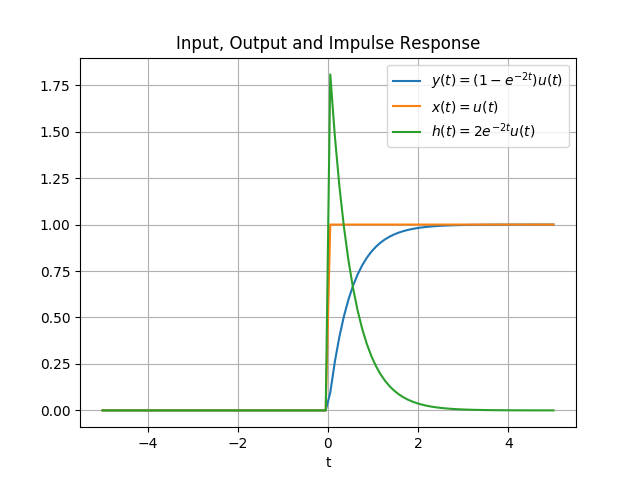
\includegraphics[width=\columnwidth]{figs/EE18BTECH11021_fig.png}
\end{figure}
\end{enumerate}
%\section{State-Space Model}
%\input{./chapters/ee18btech11004.tex}
%\subsection{Second Order System}
%\section{Nyquist Plot}
%\section{Phase Margin}
%\section{Gain Margin}
%\section{Compensators}
%\subsection{Phase Lead}
%\begin{enumerate}[label=\thesection.\arabic*.,ref=\thesection.\theenumi]
\numberwithin{equation}{enumi}

\item
What is the purpose of a phase lead compensator?

\solution 
\begin{itemize}
    \item Phase lead compensators are used to produce an output having a phase lead when an input is applied
    \item The major application is to help improve the Phase Margin (P.M) of the system.
\end{itemize}

\item
Through an example show how the compensator in Problem 7.1 can be used in a control system

Consider a control system with the Transfer Function

\begin{align}
G(s) = \frac{1}{s(3s+1)}
\end{align}
\begin{align}
G\brak{\j\omega}&=\frac{1}{\brak{j\omega}\brak{3j\omega+1}} 
\end{align}

\begin{align}
\implies 
\abs{G\brak{\j\omega}}&=\frac{1}{{\omega}{\brak{\sqrt{9\omega^2+1}}}}
\end{align}

\begin{align}
\angle G\brak{\j\omega}&=- \tan^{-1}(3\omega) - 90\degree
\end{align}

At Gain Crossover,
\begin{align}
\abs{G\brak{\j\omega}}&=1
\end{align}

\begin{align}
\implies \frac{1}{{\omega}{\brak{\sqrt{9\omega^2+1}}}} =1
\end{align}

\begin{align}
\implies \omega_{gc} = 0.531
\end{align}

\begin{align}
\angle G\brak{\j\omega} = -147.88\degree
\implies PM=32.12\degree
\end{align}
Phase Margin is only 32.12\degree which is below the acceptable range of Phase Margin i.e 45\degree.

Now we will apply Lead Compensator
\begin{align}
D(s) = \frac{3(s+\frac{1}{3T})}{(s+\frac{1}{T})}
\end{align}
Choose T = 1 for this compensator

We have,
\begin{align}
D(s) = \frac{3(s+\frac{1}{3})}{(s+1)}
\end{align}

By cascading the Compensator and the Open Loop Transfer Function, we get
\begin{align}
D(s)G(s) = \frac{1}{s(3s+1)} \frac{3(s+\frac{1}{3})}{(s+1)}
\end{align}

\begin{align}
Let G_{1}(s) = D(s)G(s)
\end{align}

\begin{align}
\implies G_{1}(s) = \frac{1}{s(s+1)}
\end{align}

Calculating Phase Margin for cascaded Transfer Function
\begin{align}
G_{1}(s) = \frac{1}{s(s+1)}
\end{align}
\begin{align}
G_{1}\brak{\j\omega}&=\frac{1}{\brak{j\omega}\brak{j\omega+1}} 
\end{align}

\begin{align}
\implies 
\abs{G_{1}\brak{\j\omega}}&=\frac{1}{{\omega}{\brak{\sqrt{\omega^2+1}}}}
\end{align}

\begin{align}
\angle G_{1}\brak{\j\omega}&=- \tan^{-1}(\omega) - 90\degree
\end{align}

At Gain Crossover,
\begin{align}
\abs{G_{1}\brak{\j\omega}}&=1
\end{align}

\begin{align}
\implies \frac{1}{{\omega}{\brak{\sqrt{\omega^2+1}}}} =1
\end{align}

\begin{align}
\implies \omega_{gc} = 0.786
\end{align}

\begin{align}
\angle G\brak{\j\omega} = -128.167\degree
\implies PM=51.83\degree
\end{align}

As we can see, the Phase Margin has gone above 45\degree which is the acceptable range of Phase Margin.

Therefore, through this example we have shown that a Lead Compensator is helpful in improving the Phase Margin of the System.

\item Verify the above improvement in Phase Margin with the help of a Python Code
\solution
\begin{lstlisting}
codes/EE18BTECH11021_2.py
\end{lstlisting}

\begin{figure}
\centering
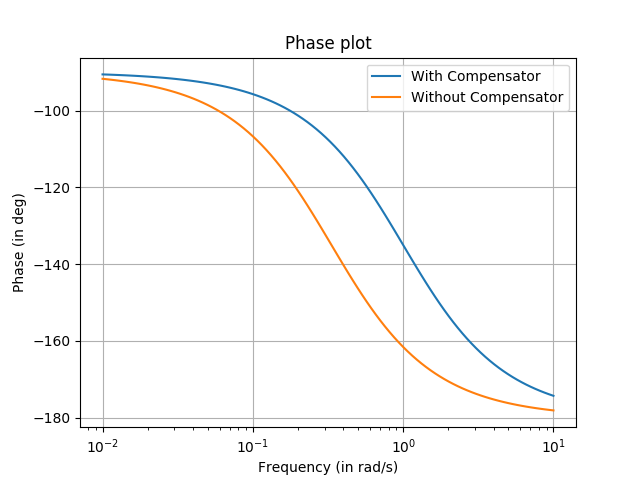
\includegraphics[width=\columnwidth]{figs/EE18BTECH11021_fig_2.png}
\end{figure}

%\section{Oscillator}
\section{Controllers}
\begin{enumerate}[label=\thesection.\arabic*.,ref=\thesection.\theenumi]
\numberwithin{equation}{enumi}

\item
Write the general expression for the trasfer function of a PID controller.

\solution
The Transfer Function of the PID Controller is
\begin{align}
    K_{p}\brak{1 + T_{d}s + \frac{1}{T_{i}s}}
\end{align}

\item
Write the general expression for the trasfer function of a PD controller.

\solution
PD Controllers are special cases of PID Controllers in which only Proportional and Derivative Controls are used.

The Transfer Function of PD Controller is 
\begin{align}
    K_{p}(1 + T_{d}s)
\end{align}

\item
Write the general expression for the transfer function of a PI controller.

\solution
PD Controllers are special cases of PID Controllers in which only Proportional and Integral Controls are used.

The Transfer Function of PI Controller is 
\begin{align}
    K_{p}\brak{1 +  \frac{1}{T_{i}s}}
\end{align}


\item
For a unity Feedback system 
\begin{align}
    G(s) = \frac{K}{s(s+2)(s+4)(s+6)}
\end{align}


Design a PD Controller with $K_{v} = 2$ and Phase Margin 30\degree

\solution
PD Controller is cascaded with the given G(s).
The Transfer Function of the PD Controller is $K_{p}(1 + T_{d}s)$

\begin{align}
    G_{c}(s) = \frac{K_{p}(1 + T_{d}s)K}{s(s+2)(s+4)(s+6)}
\end{align}

\begin{align}
    K_{v} = \lim_{s \to 0} sG_{1}(s) = 2
\end{align}

If we choose $K_{p} = 1$
\begin{align}
    \implies K = 96
\end{align}

For Phase Margin 30\degree, at Gain Crossover Frequency w

\begin{align}
    \tan^{-1}\brak{T_{d}\omega} - \tan^{-1}\brak{\frac{\omega}{2}} - \tan^{-1}\brak{\frac{\omega}{4}}
    \tan^{-1}\brak{\frac{\omega}{6}} = -60
\end{align}

\begin{align}
    \abs{G_{1}\brak{\j\omega}} = \frac{96\sqrt{T_{d}^2w^2 + 1}}{w\sqrt{(w^2+4)(w^2 + 16)(w^2 + 36)}} = 1
\end{align}

By Hit and Trial, one of the best combinations is
\begin{align}
    w = 4
\end{align}
\begin{align}
    T_{d} = 1.884
\end{align}
We get a Phase Margin of 30.31\degree

\item
Verify using a Python Plot

\solution
\begin{lstlisting}
codes/EE18BTECH11021_3.py
\end{lstlisting}

\begin{figure}
\centering
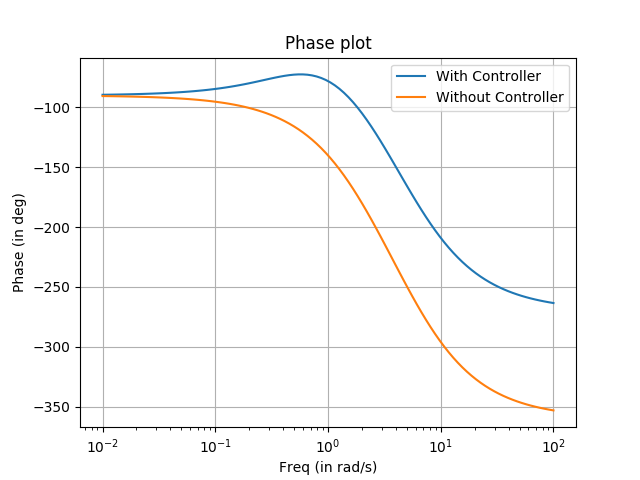
\includegraphics[width=\columnwidth]{figs/EE18BTECH11021_PD.png}
\end{figure}

\item
Design a PI Controller with $K_{v} = \infty$ and Phase Margin 30\degree

\solution
PI Controller is cascaded with the given G(s).
The Transfer Function of the PI Controller is $K_{p}\brak{1 + \frac{1}{T_{i}s}}$

\begin{align}
    G_{1}(s) = \frac{K_{p}\brak{1 +  \frac{1}{T_{i}s}}K}{s(s+2)(s+4)(s+6)}
\end{align}

Choose $K_{p}K = 96$
This can be written as
\begin{align}
    G_{1}(s) = \frac{96(T_{i}s + 1)}{T_{i}s^2(s+2)(s+4)(s+6)}
\end{align}

For Phase Margin 30\degree, at Gain Crossover Frequency w

\begin{align}
    \tan^{-1}(T_{i}\omega) - \tan^{-1}\brak{\frac{\omega}{2}} - \tan^{-1}\brak{\frac{\omega}{4}}
    \tan^{-1}\brak{\frac{\omega}{6}} = 30
\end{align}

\begin{align}
    \abs{G_{1}\brak{\j\omega}} = \frac{96\sqrt{T_{i}^2w^2 + 1}}{T_{i}^2w^2\sqrt{(w^2+4)(w^2 + 16)(w^2 + 36)}} = 1
\end{align}

By Hit and Trial, one of the best combinations is
\begin{align}
    w = 0.75
\end{align}
\begin{align}
    T_{i} = 2.713
\end{align}
We get a Phase Margin of 25.53\degree

\item
Verify using a Python Plot

\solution
\begin{lstlisting}
codes/EE18BTECH11021_4.py
\end{lstlisting}

\begin{figure}
\centering
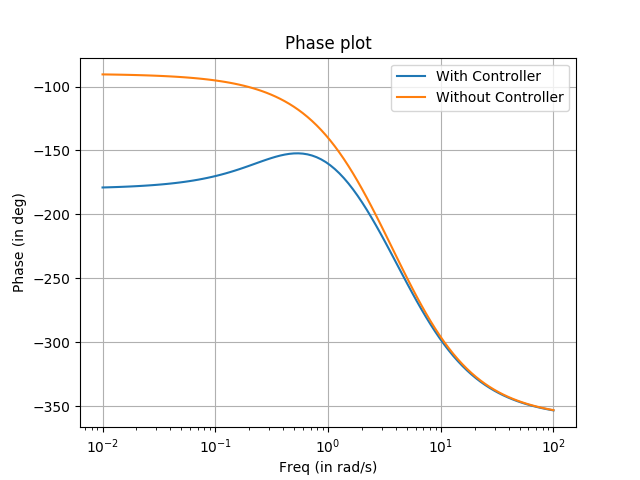
\includegraphics[width=\columnwidth]{figs/EE18BTECH11021_PI.png}
\end{figure}

\item
Design a PID Controller with $K_{v} = \infty$ and Phase Margin 30\degree

\solution
PID Controller is cascaded with the given G(s).
The Transfer Function of the PD Controller is $K_{p}\brak{1 + T_{d}s + \frac{1}{T_{i}s}}$

\begin{align}
    G_{1}(s) = \frac{K_{p}\brak{1 + T_{d}s + \frac{1}{T_{i}s}}K}{s(s+2)(s+4)(s+6)}
\end{align}

Choose $K_{p}K = 96$
This can be written as
\begin{align}
    G_{1}(s) = \frac{96(T_{i}T_{d}s^2 + T_{i}s +  1)}{T_{i}s^2(s+2)(s+4)(s+6)}
\end{align}

For Phase Margin 30\degree, at Gain Crossover Frequency w

\begin{align}
    \tan^{-1}(\frac{T_{i}\omega}{1-T{i}T_{d}w^2}) - \tan^{-1}\brak{\frac{\omega}{2}} - \tan^{-1}\brak{\frac{\omega}{4}}
    \tan^{-1}\brak{\frac{\omega}{6}} = 30
\end{align}

\begin{align}
    \abs{G_{1}\brak{\j\omega}} = \frac{96\sqrt{(1-T{i}T_{d}w^2)^2 + T_{i}^2}}{T_{i}^2w^2\sqrt{(w^2+4)(w^2 + 16)(w^2 + 36)}} = 1
\end{align}

By Hit and Trial, one of the best combinations is
\begin{align}
    w = 1
\end{align}
\begin{align}
    T_{i} = 1.738
\end{align}
\begin{align}
    T_{d} = 0.4
\end{align}
We get a Phase Margin of 30\degree

\item
Verify using a Python Plot

\solution
\begin{lstlisting}
codes/EE18BTECH11021_5.py
\end{lstlisting}

\begin{figure}
\centering
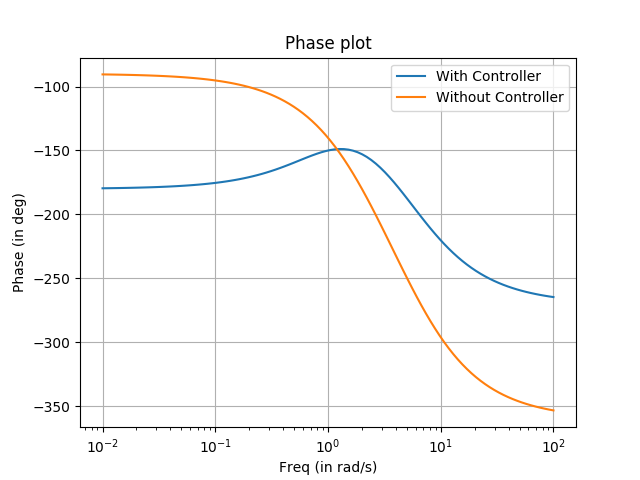
\includegraphics[width=\columnwidth]{figs/EE18BTECH11021_PID.png}
\end{figure}
\end{document}